\section{From the linear seed to a nonlinear solution}
\label{sec:solving-the-equation}
\label{sec:exact-return-height}

We can now explain why the unknowns were chosen as in
Table~\ref{tab:unknowns}, and solve the system. The height solves the
curvature equation. The compact metric parameter $\nu$ removes its
obstruction in the second mode. One control $\kappa_m$ per negative
component adjusts the mean travel angle, and the odd charts adjust the
oscillating part of the return maps; these two tasks are separated by
taking the angular mean. The return residual depends on the height
only through $qu$, so the feedback from the return equations to the
height equation carries the small factor $q$, and the coupled linear
system is solved by a perturbation of a triangular one.

Objects of the full system are written in bold type: the state $\bx$,
the residual $\mathbf R$, the approximate inverse $\mathbf V$ and the
error $\mathbf Q$.

\subsection{The residual and its derivative}

For a state $\bx=(u,\nu,\kappa,h_L)$ as in
\eqref{eq:rewrite-state} and a parameter $q\in\R$ let
\begin{equation}\label{eq:readable-joint-residual}
 \mathbf R(\bx,q)=(\mathcal A,\mathfrak e),
 \qquad \mathcal A=\mathcal F_q(w,u),
 \qquad \mathfrak e=\mathfrak e(qu,\kappa,h_L),
\end{equation}
where $w$ is the profile \eqref{eq:full-height-metric-controls} and
$\mathfrak e=(\mathfrak e_m)_m$ is the return residual
\eqref{eq:full-height-one-chart} on every negative component. The
return residual depends on the height through $Z=qu$, on $\kappa$ and
on $h_L$; it does not depend on $\nu$ or on the endpoint constant of
$u$, because $\chi_*$ and the derivative of $\chi_L$ are supported in
positive components. The spaces of increments and of residuals are
\[
 \mathfrak X=(\mathcal X_\beta\cap\ker\ell_*)\times\R
       \times\mathcal K_\beta\times\mathcal Z_{\beta,\mathrm{odd}},
 \qquad
 \mathfrak Y=\mathcal Y_\beta\times\mathcal Z_{\beta,\mathrm{even}} .
\]
The second factor of $\mathfrak Y$ includes the angular means; the
first incorporates the conservation law of
Lemma~\ref{lem:scalar-integral}. By \eqref{eq:normalized-integral}
and the calculus of Section~\ref{sec:fixed-geometry}, $\mathbf R$ is a
smooth tame map into $\mathfrak Y$ on the open set
$\mathfrak n_{b_0}<\epsilon_0$. It vanishes at
\[
 q=0,\qquad \bx_0=(\Phi_*,0,0,\id),
\]
since $\mathscr L_{w_*}\Phi_*=0$ and the return maps of the reference
profile are the rotations $R_{\pm T_m}$.

\paragraph{The derivative of the return residual.}
Write
\begin{equation}\label{eq:joint-circle-linear-rows}
 C_{\bx}^{\circ}=D_Z\mathfrak e,\qquad
 R_{\bx}^{\circ}=\av{C_{\bx}^{\circ}},\qquad
 \mathcal D_{\bx}=D_\kappa\mathfrak e,\qquad
 \mathsf J_{\bx}=\av{\mathcal D_{\bx}} .
\end{equation}
The residual on the component $m$ depends only on the height near
that component, on its chart and on $\kappa_m$. So $\mathsf J_{\bx}$
is a diagonal matrix. At a state with radial height and trivial
charts, $\mathfrak e_m=T_m(w)-T_m(w_*)$, and by the normalization of
the controls in Lemma~\ref{lem:quantitative-optical-controls},
$\mathsf J=I$ at the reference. On a neighbourhood of low order the
entries of $\mathsf J_{\bx}$ stay uniformly away from zero, and
$\mathsf J_{\bx}^{-1}$ is smooth tame.

At the reference state, the mean $R_0^\circ$ of the derivative with
respect to the height annihilates all nonzero angular frequencies, by
invariance under rotation, and on a radial increment $Z$ it is
\begin{equation}\label{eq:rewrite-reference-circle-row}
 (R_0^\circ Z)_m
 =-\int v_0\,\frac{1+w_*^2}{w_*}\,Z_r\,dr ,
\end{equation}
the integral being over the $m$th negative component. Indeed, for a
radial height $h+Z$ the characteristic speed
\eqref{eq:completed-characteristics} is
$v_0\,w_*\sqrt D/(w_*+Z_r)$ with $D=1-2w_*Z_r-Z_r^2$, and its
logarithmic derivative at $Z=0$ is $-(1+w_*^2)Z_r/w_*$. In particular
$R_0^\circ\Phi_*=0$.

\paragraph{The corrected linear system.}
Let $K_{\bx}=D_\kappa\mathcal A$ and, as before,
$k_{\bx}=D_\nu\mathcal A$. For an increment
$(\eta,\mu,\varkappa,\psi\circ h_L)$ of the state
$(u,\nu,\kappa,h_L)$ and a right side $(f,g)\in\mathfrak Y$ we
consider
\begin{equation}\label{eq:corrected-coupled-linear-system}
 \begin{split}
 \widehat L_{\bx}\eta+k_{\bx}\,\mu+K_{\bx}\,\varkappa&=f,
                    \qquad \ell_*\eta=0,\\
 q\,C_{\bx}^{\circ}\eta+\mathcal D_{\bx}\,\varkappa
                            +\mathcal M_T\psi&=g .
 \end{split}
\end{equation}
This is the derivative of $\mathbf R$ with respect to the state,
except for three terms that have been dropped: the two residual
corrections in \eqref{eq:readable-completed-height-derivative} and the
term $\mathcal Q_h$ in \eqref{eq:full-height-chart-derivative}. Each
of them is proportional to $\mathcal A$ or to $\mathfrak e$. The
structure of the system is shown in Figure~\ref{fig:coupled-columns}.

\begin{figure}[htbp]
\centering
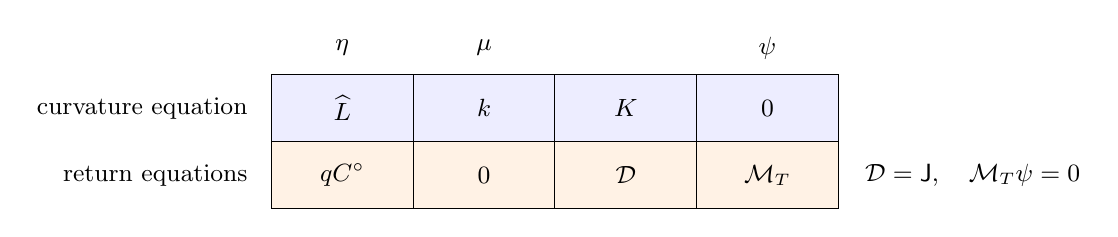
\begin{tikzpicture}[x=1.8cm,y=.85cm,font=\small]
\fill[blue!7] (0,1) rectangle (4,2);
\fill[orange!10] (0,0) rectangle (4,1);
\draw (0,0) rectangle (4,2);
\draw (0,1)--(4,1);
\foreach \x in {1,2,3} {\draw (\x,0)--(\x,2);}
\node at (.5,2.4) {$\eta$}; \node at (1.5,2.4) {$\mu$};
\node at (2.5,2.4) {$\varkappa$}; \node at (3.5,2.4) {$\psi$};
\node at (.5,1.5) {$\widehat L$}; \node at (1.5,1.5) {$k$};
\node at (2.5,1.5) {$K$}; \node at (3.5,1.5) {$0$};
\node at (.5,.5) {$qC^\circ$}; \node at (1.5,.5) {$0$};
\node at (2.5,.5) {$\mathcal D$}; \node at (3.5,.5) {$\mathcal M_T$};
\node[anchor=east] at (-.1,1.5) {curvature equation};
\node[anchor=east] at (-.1,.5) {return equations};
\node[anchor=west] at (4.12,.5)
 {$\av{\mathcal D}=\mathsf J,\quad\av{\mathcal M_T\psi}=0$};
\end{tikzpicture}
\caption{The corrected linear system and its four columns: the
increments $\eta,\mu,\varkappa,\psi$ of the height, of $\nu$, of the
controls $\kappa$ and of the charts. Taking the mean of the second
row removes the chart column. The feedback from the second row to the
height is multiplied by $q$.}
\label{fig:coupled-columns}
\end{figure}

\subsection{The control column gains all coefficient weights}

Let $G_{\bx}$ be the inverse of
Proposition~\ref{prop:rewrite-volume-inverse} and put
$U_{\bx}=G_{\bx}K_{\bx}$: the response $(\eta,\mu)$ of the first
equation to an increment of the controls. The natural space for
increments of the controls is
\[
 B_\beta=\Bigl\{\varkappa=(\varkappa_m):\
 \|\varkappa\|_{B_\beta}^2=\sum_mH_m^{-2\beta}|\varkappa_m|^2<\infty\Bigr\},
\]
which has no weight $M$ at all.

\begin{lemma}[Smoothing by the control column]\label{lem:control-smoothing}
For every $s$, with a fixed loss $d_*$,
\begin{equation}\label{eq:weak-control-smoothing}
 \|K_{\bx}\varkappa\|_{\mathcal Y_\beta,s}
 +\|U_{\bx}\varkappa\|_{\mathcal X_\beta,s}+|(U_{\bx}\varkappa)_{\mu}|
 \le C_s\,(1+\mathfrak n_{s+d_*})\,\|\varkappa\|_{B_\beta} ,
\end{equation}
where the middle term is the norm of the height component of
$U_{\bx}\varkappa$ and the last term is its scalar component.
\end{lemma}

\begin{proof}
\step{1: two decaying factors}
Differentiating the formula \eqref{eq:normalized-integral} for
$\mathcal F_q$ with respect to the controls gives
\[
 K_{\bx}\varkappa=\int_0^1D_\kappa\bigl[\,r\,D_z\mathcal N_{h}(h+tqu)\bigr]
 [\varkappa]\;u\,dt ,
\]
where $h'=w$ and the derivative $D_\kappa$ acts on $w$ and on $h$.
Every term of the result contains the increment of the control and a
derivative of positive order of the height $u$: the curvature
residual does not change when a constant is added to the height. This is true also at $q=0$, where
the derivative is that of $\mathscr L_wu$. On the component $m$ write
$\varkappa_m=H_m^\beta b_m$. The derivative of the height contributes
another factor $H_m^\beta$; the endpoint constant of $u$ does not
contribute, because the supports of the controls lie in negative
components. After division by the weight $H_m^\beta$ of the source
space a factor $H_m^\beta$ remains.

\step{2: summation}
At the order $s$, all coordinate, cutoff and reciprocal factors and
the derivatives of the control $\chi_m$ together cost a coefficient
power $\mathcal E_m^{C_s}$ and a fixed power of $M_m$; the remaining
factor $H_m^\beta$ bounds their product, by
\eqref{eq:full-material-envelope}. The product estimate
\eqref{eq:weighted-product} puts one factor of the state at the high
order. The supports of the controls are disjoint, so summing over $m$
gives the bound for $K_{\bx}$ with $(\sum_m|b_m|^2)^{1/2}
=\|\varkappa\|_{B_\beta}$. Composition with $G_{\bx}$ adds its fixed
loss.
\end{proof}

\subsection{Solving the corrected system}

\begin{proposition}[The approximate right inverse]\label{prop:approx-inverse}
After $\epsilon_0$ and the range of $q$ have been decreased, the
system \eqref{eq:corrected-coupled-linear-system} has for every
$(f,g)\in\mathfrak Y$ the solution
\begin{equation}\label{eq:joint-height-circle-inverse}
 \begin{split}
 \varkappa&=(I-q\,\mathsf J^{-1}R^\circ U)^{-1}\,
         \mathsf J^{-1}\,\bigl(\av g-q\,R^\circ Gf\bigr),\\
 (\eta,\mu)&=Gf-U\varkappa,\\
 \psi&=\mathcal M_T^{-1}\bigl(g-q\,C^\circ\eta-\mathcal D\varkappa\bigr),
 \end{split}
\end{equation}
where the subscript $\bx$ is omitted and $R^\circ$, $C^\circ$ act on
the height component of $G$ and $U$. The map
\[
 \mathbf V(\bx,q)\,(f,g)=(\eta,\mu,\varkappa,\psi\circ h_L)
\]
is smooth tame, and linear in $(f,g)$.
\end{proposition}

\begin{proof}
\step{1: elimination}
The first row gives $(\eta,\mu)=Gf-U\varkappa$. Taking the angular
mean of the second row removes $\mathcal M_T\psi$ and gives
\[
 (I-q\,\mathsf J^{-1}R^\circ U)\,\varkappa
              =\mathsf J^{-1}\,\bigl(\av g-q\,R^\circ Gf\bigr).
\]
By Lemma~\ref{lem:control-smoothing}, $R^\circ U$ is a bounded
operator from $B_\beta$ to the \emph{same} space $B_\beta$, with norm
controlled by finitely many norms of the state. Choose the
neighbourhood so that these norms are bounded, and then $|q|$ so small
that $\|q\,\mathsf J^{-1}R^\circ U\|_{B_\beta\to B_\beta}<\tfrac12$.
This gives the first line of
\eqref{eq:joint-height-circle-inverse}, and the second follows. By
the equation for $\varkappa$, the argument of $\mathcal M_T^{-1}$ in
the third line has mean zero on every component, so
\eqref{eq:rewrite-circle-inverse} applies.

\step{2: regularity}
Higher norms of $\varkappa$ are read off from the identity
\[
 \varkappa=\mathsf J^{-1}\bigl(\av g-q\,R^\circ Gf\bigr)
      +q\,\mathsf J^{-1}R^\circ U\varkappa ,
\]
satisfied by the solution already found. By
Lemma~\ref{lem:control-smoothing} the last term has all higher norms,
bounded by $\|\varkappa\|_{B_\beta}$ and one high norm of the state;
the first term has the norms of the sources with a fixed loss. So
$\varkappa$ lies in all the spaces $\mathcal K_{\beta,s}$, with tame
bounds, and substitution gives the estimates for $\eta$, $\mu$ and
$\psi$.

\step{3: smoothness}
The resolvent identity gives continuity in the base space, and the
identity of Step~2 with its estimates gives continuity in every
order. By Theorem~\ref{thm:hamilton-inverse} below, applied to the
inverse in the first line, all three formulas are smooth tame.
\end{proof}

\subsection{The quadratic error and the Nash--Moser theorem}

We use two theorems of Hamilton. Tame spaces and smooth tame maps
were defined in Section~\ref{subsec:spaces}.

\begin{theorem}[Hamilton: families of inverses]
\label{thm:hamilton-inverse}
Let $U$ be an open subset of a tame space, let
$\mathfrak H,\mathfrak K$ be tame spaces, and let
$L:U\times\mathfrak H\to\mathfrak K$ be a smooth tame map which is
linear in its second argument. Suppose that $L(x)$ is bijective for
every $x\in U$, and that the family of inverses
$(x,y)\mapsto L(x)^{-1}y$ is continuous and tame. Then this family is
smooth tame.
\end{theorem}

This is \cite[Part~II, Theorem~3.1.1]{Hamilton1982}. Existence,
uniqueness, continuity and tame bounds for the inverses are
hypotheses; the theorem supplies their derivatives. It was used in
this way in Propositions~\ref{prop:rewrite-volume-inverse}
and~\ref{prop:approx-inverse}.

\begin{theorem}[Hamilton: implicit function theorem with quadratic error]
\label{thm:hamilton-quadratic}
Let $\mathfrak X,\mathfrak P,\mathfrak Y$ be tame spaces and let
$\mathbf R:U\subset\mathfrak X\times\mathfrak P\to\mathfrak Y$ be a
smooth tame map on an open set. Suppose there are smooth tame maps
$\mathbf V(\bx,q)\,\mathbf y$ with values in $\mathfrak X$, linear in
$\mathbf y\in\mathfrak Y$, and $\mathbf Q(\bx,q)\,[\mathbf r,\mathbf y]$
with values in $\mathfrak Y$, bilinear in
$(\mathbf r,\mathbf y)\in\mathfrak Y\times\mathfrak Y$, such that
\begin{equation}\label{eq:rewrite-hamilton-hypothesis}
 D_{\bx}\mathbf R(\bx,q)\,\mathbf V(\bx,q)\,\mathbf y
        =\mathbf y+\mathbf Q(\bx,q)\,[\mathbf R(\bx,q),\mathbf y]
\end{equation}
for all $(\bx,q)\in U$ and all $\mathbf y$. Then near every zero
$(\bx_0,q_0)$ of $\mathbf R$ there is a smooth tame map
$q\mapsto\bx(q)$ with $\bx(q_0)=\bx_0$ and
$\mathbf R(\bx(q),q)=0$.
\end{theorem}

This is \cite[Part~III, Theorem~3.3.1]{Hamilton1982}. The point of
the hypothesis is that $\mathbf V$ need only be an inverse \emph{up to
an error proportional to the residual}; but the identity must hold
exactly, with the two arguments of $\mathbf Q$ independent. An
informal quadratic bound would not suffice. The theorem gives a
solution, not its uniqueness, which we do not need.

\begin{proposition}[The quadratic error identity]\label{prop:quadratic-error}
For $\mathbf r=(\mathbf r_1,\mathbf r_2)\in\mathfrak Y$ and
$\mathbf y=(f,g)\in\mathfrak Y$, let $(\eta,\mu,\varkappa,\psi)$ be
given by \eqref{eq:joint-height-circle-inverse} and define
\[
 \mathbf Q(\bx,q)\,[\mathbf r,\mathbf y]
 =\Bigl(q\,\partial_\theta\bigl(B\,\mathbf r_1\,\eta_\theta\bigr)
                   +\mathscr E_{\bx}(\mathbf r_2)\,\eta,\ \
              \mathcal Q_h(\mathbf r_2,\psi)\Bigr),
\]
where in $\mathcal Q_h$ the points of evaluation in
\eqref{eq:full-height-chart-derivative} are those of the actual state
and only the explicit factors $\mathfrak e$, $\mathfrak e'$ are
replaced by $\mathbf r_2$, $\mathbf r_2'$, as was done for
$\mathscr E_{\bx}$ in
Proposition~\ref{prop:optical-residual-completion}. Then $\mathbf Q$
is a smooth tame family of bilinear maps
$\mathfrak Y\times\mathfrak Y\to\mathfrak Y$, and
\eqref{eq:rewrite-hamilton-hypothesis} holds.
\end{proposition}

\begin{proof}
For the increments \eqref{eq:joint-height-circle-inverse}, the
identities \eqref{eq:readable-completed-height-derivative} and
\eqref{eq:full-height-chart-derivative} give the true derivative
\begin{equation}\label{eq:joint-height-circle-quadratic-error}
 D_{\bx}\mathbf R\,(\eta,\mu,\varkappa,\psi\circ h_L)
 =\Bigl(f+q\,\partial_\theta\bigl(B\,\mathcal A\,\eta_\theta\bigr)
              +\mathscr E_{\bx}(\mathfrak e)\,\eta,\ \
        g+\mathcal Q_h(\mathfrak e,\psi)\Bigr),
\end{equation}
which is \eqref{eq:rewrite-hamilton-hypothesis} with
$\mathbf r=\mathbf R=(\mathcal A,\mathfrak e)$. The increments are
linear in $\mathbf y$, so $\mathbf Q$ is bilinear.

It takes values in $\mathfrak Y$. Its first component has integral
zero: one term is an angular derivative, the other is in divergence
form with compact support inside the negative components. Its second
component is even. Finally, every term is a product of two factors
each of which decays like $H^\beta$, so by the calculus of
Section~\ref{sec:fixed-geometry} and the estimates for flows,
$\mathbf Q$ is smooth tame with values in the spaces of weight
$\beta$. All neighbourhoods of the state used here are defined by
norms of one fixed finite order; their size does not depend on the
order of the output.
\end{proof}

\begin{theorem}[The solution branch]\label{thm:weak-branch}
There are $q_1>0$ and a smooth tame map
\begin{equation}\label{eq:rewrite-weak-branch}
 q\mapsto\bx(q)=(u_q,\nu_q,\kappa_q,h_{L,q}),\qquad |q|<q_1,
\end{equation}
with $\bx(0)=(\Phi_*,0,0,\id)$ and
$\mathbf R(\bx(q),q)=0$. In particular
$u_q=\Phi_*+O(q)$ in every norm of $\mathcal X_\beta$.
\end{theorem}

\begin{proof}
We verify the hypotheses of
Theorem~\ref{thm:hamilton-quadratic} with $\mathfrak P=\R$; they are
listed in Table~\ref{tab:hamilton-hypotheses}. The order of the
choices matters. First the reference profile, the spaces and the
finite order $b_0$ are fixed; then $\epsilon_0$; then the range of
$q$, so that the control equation in
Proposition~\ref{prop:approx-inverse} can be solved. All estimates of
higher order hold on the neighbourhood so obtained, with constants
that depend on the order; no further choice is made. At a zero of
$\mathbf R$ the identity \eqref{eq:rewrite-hamilton-hypothesis} shows
that the derivative with respect to the state is surjective, with
right inverse $\mathbf V$.
\end{proof}

\begin{table}[htbp]
\centering
\begin{tabularx}{\linewidth}{@{}lY@{}}
\toprule
Hypothesis & Where it is verified\\
\midrule
Tame spaces &
 Lemma~\ref{prop:full-physical-tame}; the scalar factors and the
 affine slice $\ell_*u=1$ are tame direct summands.\\
Open domain &
 The set $\mathfrak n_{b_0}<\epsilon_0$, defined by norms of one
 finite order
 (Lemma~\ref{lem:common-geometric-neighborhood},
 Proposition~\ref{prop:uniform-physical-geometry}).\\
$\mathbf R$ smooth tame, with values in $\mathfrak Y$ &
 Formula \eqref{eq:normalized-integral} and
 Lemma~\ref{lem:scalar-integral} for $\mathcal A$; the calculus of
 Lemmas~\ref{lem:one-high-factor}, \ref{lem:circle-flow}
 and~\ref{lem:current-geometric-jets} for $\mathfrak e$.\\
A zero &
 $(\bx_0,0)$: $\mathscr L_{w_*}\Phi_*=0$, $\ell_*\Phi_*=1$, and the
 reference return maps are rotations.\\
$\mathbf V$ smooth tame and linear &
 Proposition~\ref{prop:approx-inverse}, which rests on
 Proposition~\ref{prop:rewrite-volume-inverse}.\\
$\mathbf Q$ smooth tame and bilinear &
 Proposition~\ref{prop:quadratic-error}, with
 Proposition~\ref{prop:optical-residual-completion} for
 $\mathscr E_{\bx}$.\\
The identity \eqref{eq:rewrite-hamilton-hypothesis} &
 \eqref{eq:joint-height-circle-quadratic-error}.\\
\bottomrule
\end{tabularx}
\caption{The hypotheses of Theorem~\ref{thm:hamilton-quadratic} and
where they are verified.}
\label{tab:hamilton-hypotheses}
\end{table}


This solves the nonlinear system in the scale of weight $\beta$. The
next section extracts stronger information from the equations
themselves, without a second iteration in another space.
